\documentclass[10pt]{article}
\usepackage[margin=2cm]{geometry}
\usepackage{booktabs,graphicx,amsmath,amssymb}
\usepackage[T1]{fontenc}
\usepackage{url}
\usepackage{mathptmx}
\graphicspath{{../figures/}{figures/}}
\renewcommand{\thetable}{S\arabic{table}}
\renewcommand{\thefigure}{S\arabic{figure}}
\title{Supplementary material\\[4pt]\large Lesion-level leakage and site-level reliability in Fed-ISIC2019}
\date{}
\begin{document}
\maketitle
All tables are generated by \texttt{scripts/make\_supplement.py} from the result files in the code repository
(\url{https://github.com/Sisty37/reliable-fed-derm}).
\section*{S1. Data and split audit}
Lesion identifiers come from the HAM10000 metadata (clients 1, 2, 3, 5) and the ISIC 2019 metadata (clients 0, 4). Checks on all 23,247 images: missing identifiers 0, identifiers equal to the image name 0, lesions with more than one diagnosis 0, lesions with images in two clients 9 (all in clients 1 and 2, both from the Vienna institution), sum of per-client lesion counts 11,856 versus 11,847 distinct lesions. Patient identifiers are not available.
\begin{table*}[!htbp]
\centering
\footnotesize
\caption{Clients, sources and lesion multiplicity (images per lesion).}
\label{tab:s1prov}
\begin{tabular}{@{}llp{2.6cm}rrrrrrr@{}}
\toprule
Client & Source & Lesion IDs from & Images & Lesions & Mean & $\ge2$ img. & Median & P90 & Max \\
\midrule
0 & BCN20000 & ISIC 2019 metadata & 12,413 & 3,576 & 3.47 & 3,088 & 3 & 6 & 31 \\
1 & HAM vidir\_molemax & HAM10000 metadata & 3,954 & 3,954 & 1.00 & 0 & 1 & 1 & 1 \\
2 & HAM vidir\_modern & HAM10000 metadata & 3,363 & 1,695 & 1.98 & 1,261 & 2 & 3 & 6 \\
3 & HAM rosendahl & HAM10000 metadata & 2,259 & 1,552 & 1.46 & 572 & 1 & 2 & 5 \\
4 & MSK & ISIC 2019 metadata & 819 & 801 & 1.02 & 15 & 1 & 1 & 4 \\
5 & HAM vienna\_dias & HAM10000 metadata & 439 & 278 & 1.58 & 122 & 1 & 3 & 4 \\
\bottomrule
\end{tabular}
\end{table*}
\begin{table*}[!htbp]
\centering
\footnotesize
\caption{Images/lesions per client and class (all data).}
\label{tab:s1cls}
\begin{tabular}{@{}lrrrrrrrr@{}}
\toprule
Client & MEL & NV & BCC & AK & BKL & DF & VASC & SCC \\
\midrule
0 & 2857/524 & 4206/1281 & 2809/983 & 737/236 & 1138/353 & 124/40 & 111/37 & 431/122 \\
1 & 24/24 & 3720/3720 & 2/2 & -- & 124/124 & 30/30 & 54/54 & -- \\
2 & 680/330 & 1832/928 & 211/110 & 21/12 & 475/246 & 51/25 & 82/39 & 11/5 \\
3 & 342/225 & 803/538 & 296/211 & 109/76 & 490/349 & 30/16 & 3/2 & 186/135 \\
4 & 215/201 & 415/411 & -- & -- & 189/189 & -- & -- & -- \\
5 & 67/44 & 350/217 & 5/4 & -- & 10/8 & 4/2 & 3/3 & -- \\
\bottomrule
\end{tabular}
\end{table*}
\begin{table*}[!htbp]
\centering
\scriptsize
\caption{Image-level re-splits: mean train/validation/test images per client and class (five seeds).}
\label{tab:s1splitimage}
\begin{tabular}{@{}lrrrrrrrr@{}}
\toprule
Client & MEL & NV & BCC & AK & BKL & DF & VASC & SCC \\
\midrule
0 & 2051/235/571 & 3051/314/841 & 2045/202/562 & 540/50/147 & 817/93/228 & 92/7/25 & 79/10/22 & 303/42/86 \\
1 & 17/2/5 & 2681/295/744 & 2/0/0 & -- & 88/11/25 & 21/3/6 & 38/5/11 & -- \\
2 & 492/52/136 & 1311/155/366 & 156/13/42 & 15/2/4 & 344/36/95 & 38/3/10 & 59/7/16 & 9/0/2 \\
3 & 242/32/68 & 582/60/161 & 210/27/59 & 77/10/22 & 351/41/98 & 23/1/6 & 2/0/1 & 136/13/37 \\
4 & 155/17/43 & 299/33/83 & -- & -- & 135/16/38 & -- & -- & -- \\
5 & 47/7/13 & 253/27/70 & 4/0/1 & -- & 8/0/2 & 2/1/1 & 2/0/1 & -- \\
\bottomrule
\end{tabular}
\end{table*}
\begin{table*}[!htbp]
\centering
\scriptsize
\caption{Lesion-level re-splits: mean train/validation/test images per client and class (five seeds).}
\label{tab:s1splitlesion}
\begin{tabular}{@{}lrrrrrrrr@{}}
\toprule
Client & MEL & NV & BCC & AK & BKL & DF & VASC & SCC \\
\midrule
0 & 2035/251/571 & 3033/332/841 & 2041/206/562 & 539/51/147 & 811/99/228 & 86/13/25 & 81/8/22 & 319/26/86 \\
1 & 19/2/3 & 2680/296/744 & 2/0/0 & -- & 88/11/25 & 22/2/6 & 37/6/11 & -- \\
2 & 488/60/132 & 1319/147/366 & 154/15/42 & 15/2/4 & 344/36/95 & 38/3/10 & 59/7/16 & 9/1/1 \\
3 & 246/28/68 & 575/67/161 & 212/25/59 & 74/13/22 & 357/35/98 & 21/3/6 & 1/0/2 & 138/11/37 \\
4 & 153/19/43 & 299/33/83 & -- & -- & 137/14/38 & -- & -- & -- \\
5 & 50/4/13 & 253/27/70 & 4/0/1 & -- & 7/1/2 & 2/0/2 & 2/0/1 & -- \\
\bottomrule
\end{tabular}
\end{table*}
\begin{table}[!htbp]
\centering
\footnotesize
\caption{Realized split sizes.}
\label{tab:s1sizes}
\begin{tabular}{@{}lrrrrrrr@{}}
\toprule
Split & Seed & Train img. & Val img. & Test img. & Train les. & Val les. & Test les. \\
\midrule
image & 0 & 16,731 & 1,868 & 4,648 & 9,349 & 1,038 & 3,764 \\
image & 1 & 16,775 & 1,824 & 4,648 & 9,321 & 1,035 & 3,775 \\
image & 2 & 16,773 & 1,826 & 4,648 & 9,372 & 1,040 & 3,770 \\
image & 3 & 16,788 & 1,811 & 4,648 & 9,349 & 1,038 & 3,748 \\
image & 4 & 16,828 & 1,771 & 4,648 & 9,357 & 1,039 & 3,782 \\
lesion & 0 & 16,733 & 1,871 & 4,643 & 8,468 & 940 & 2,439 \\
lesion & 1 & 16,819 & 1,782 & 4,646 & 8,533 & 946 & 2,368 \\
lesion & 2 & 16,706 & 1,898 & 4,643 & 8,516 & 945 & 2,386 \\
lesion & 3 & 16,769 & 1,835 & 4,643 & 8,510 & 944 & 2,393 \\
lesion & 4 & 16,712 & 1,892 & 4,643 & 8,533 & 947 & 2,367 \\
\bottomrule
\end{tabular}
\end{table}
\begin{table}[!htbp]
\centering
\footnotesize
\caption{Leakage of image-level test images (\%): lesion with training images in the same client, only in another client, or only in the validation fold (temperature scaling only). Lesion-grouped re-splits: maximum leakage 0.0\%.}
\label{tab:s1leak}
\begin{tabular}{@{}llrrrr@{}}
\toprule
Split & Client & Test img. & Same client & Other client only & Validation only \\
\midrule
Official & 0 & 2483 & 92.7 & 0.0 & 0.0 \\
 & 1 & 791 & 0.0 & 0.1 & 0.0 \\
 & 2 & 672 & 71.7 & 0.7 & 0.0 \\
 & 3 & 452 & 49.3 & 0.0 & 0.0 \\
 & 4 & 164 & 3.0 & 0.0 & 0.0 \\
 & 5 & 88 & 55.7 & 0.0 & 0.0 \\
 & all & 4650 & 65.8 & 0.1 & 0.0 \\
\midrule
Re-splits & 0 & 2482 & 83.0 & 0.0 & 8.9 \\
 & 1 & 791 & 0.0 & 0.2 & 0.0 \\
 & 2 & 671 & 67.9 & 0.1 & 7.8 \\
 & 3 & 452 & 43.5 & 0.0 & 4.9 \\
 & 4 & 164 & 2.7 & 0.0 & 0.7 \\
 & 5 & 88 & 50.2 & 0.0 & 6.8 \\
 & all & 4648 & 59.4 & 0.1 & 6.5 \\
\bottomrule
\end{tabular}
\end{table}
\section*{S2. Implementation details}
\begin{itemize}
\item \textbf{Model A:} EfficientNet-B0 (efficientnet-pytorch, ImageNet weights), new 8-class linear output layer;
FedAvg, FedProx, SCAFFOLD, FedBN and FedPer: 9 rounds $\times$ 100 local SGD steps (batch 64, learning rate 0.01, mixed
precision); pooled and local-only: Adam, learning rate $5\times10^{-4}$, batch 64, 20 epochs; weighted focal loss
($\gamma=2$) with FLamby's fixed class weights (5.58, 2.05, 7.02, 26.12, 9.54, 101.07, 92.52, 38.34 for MEL, NV, BCC, AK,
BKL, DF, VASC, SCC).
\item \textbf{Aggregation:} all trainable parameters averaged with weights proportional to training images.
Batch-normalization running statistics are buffers and stay with each client in every method; FedBN keeps the
batch-normalization weights and biases local as well; FedPer (model A) keeps the output layer local.
\item \textbf{Evaluation model:} global methods are evaluated with the copy of the first participating client,
including its running statistics (FLamby convention); personalized methods with each client's own model; LOCO
models apply the running statistics of the first participating client, with no adaptation to the held-out client.
\item \textbf{Frozen encoders:} embeddings in evaluation mode, fp16; one plain view and five augmented views per image
(seed $1{,}000{,}003\,v+i$); centering with the federated training mean (training fold only, all five views,
held-out client excluded for LOCO); heads with PyTorch default initialization (Kaiming-uniform weights); FedAvg-type
heads: 9 rounds $\times$ $U=6{,}400$ SGD steps; FedAvg-FT: three local SGD steps from the final FedAvg head.
\item \textbf{Temperature scaling:} per-client NLL-optimal temperature on validation lesions (grid of 600 values from
0.05 to 20), global temperature = their mean weighted by validation images.
\item \textbf{Conformal histograms:} 1,000 equal-width bins on $[0,1]$; the threshold is the upper edge of the bin in
which the cumulative count reaches the required rank (conservative).
\item \textbf{Bootstraps:} test lesions resampled with replacement within each seed's test set; all models and methods
of a seed share the replicate; seeds averaged inside each replicate.
\end{itemize}
\section*{S3. Apparent inflation per client and dose--response sensitivity}
\begin{table}[!htbp]
\centering
\footnotesize
\caption{Model A: per-client apparent inflation (BA points, five seeds; no standardization).}
\label{tab:s3A}
\begin{tabular}{@{}lrrrrrr@{}}
\toprule
Method & 0 & 1 & 2 & 3 & 4 & 5 \\
\midrule
FedAvg & 10.0 & 0.0 & $-$2.5 & 0.6 & 0.2 & 1.9 \\
FedProx & 9.5 & 0.0 & $-$1.2 & 0.7 & $-$0.2 & 5.2 \\
SCAFFOLD & 9.8 & 0.0 & 0.0 & $-$2.6 & 0.3 & $-$4.6 \\
FedBN & 11.3 & 0.0 & $-$1.3 & $-$0.3 & 0.1 & $-$0.7 \\
FedAvg-FT & 11.0 & 0.0 & $-$2.6 & 0.8 & $-$0.1 & 0.4 \\
Pooled & 22.2 & 0.0 & 1.4 & 4.3 & 0.5 & 5.7 \\
Local-only & 21.7 & 0.0 & 4.7 & 8.2 & 0.3 & 3.9 \\
FedPer & 12.1 & 0.0 & 0.7 & 2.9 & 0.4 & 11.5 \\
\midrule
Leakage rate (\%) & 83.0 & 0.2 & 68.0 & 43.5 & 2.7 & 50.2 \\
New-lesion images & 421 & 789 & 214 & 255 & 160 & 44 \\
\bottomrule
\end{tabular}
\end{table}
\begin{table}[!htbp]
\centering
\footnotesize
\caption{Model B: per-client apparent inflation (BA points, five seeds; no standardization).}
\label{tab:s3B}
\begin{tabular}{@{}lrrrrrr@{}}
\toprule
Method & 0 & 1 & 2 & 3 & 4 & 5 \\
\midrule
FedAvg & 12.0 & 0.0 & 1.5 & 0.2 & $-$0.0 & 1.4 \\
FedProx & 11.4 & 0.0 & 1.6 & 0.2 & $-$0.0 & 1.4 \\
SCAFFOLD & 11.7 & 0.0 & 2.0 & $-$0.2 & $-$0.2 & 1.5 \\
FedAvg-FT & 12.1 & 0.0 & 1.8 & 0.3 & $-$0.1 & $-$0.1 \\
Pooled & 7.5 & 0.0 & $-$0.7 & $-$2.5 & 0.2 & 2.4 \\
Local-only & 8.7 & 0.0 & 0.6 & $-$0.3 & $-$0.1 & 1.9 \\
FedPer & 20.2 & 0.0 & 1.0 & 2.9 & $-$0.6 & 8.8 \\
\midrule
Leakage rate (\%) & 83.0 & 0.2 & 68.0 & 43.5 & 2.7 & 50.2 \\
New-lesion images & 421 & 789 & 214 & 255 & 160 & 44 \\
\bottomrule
\end{tabular}
\end{table}
\begin{table}[!htbp]
\centering
\footnotesize
\caption{Weighted least-squares slope of per-client inflation on leakage rate (points per 100\% leakage): all six clients, without client 0, and range when any one client is left out.}
\label{tab:s3dr}
\begin{tabular}{@{}llrrr@{}}
\toprule
Model & Method & All & Without 0 & Leave-one-out range \\
\midrule
A & FedAvg & 8.1 & $-$1.9 & $-$1.9 to 11.5 \\
A & FedProx & 8.3 & $-$0.1 & $-$0.1 to 11.6 \\
A & SCAFFOLD & 8.2 & $-$2.2 & $-$2.2 to 13.6 \\
A & FedBN & 9.5 & $-$1.6 & $-$1.6 to 14.1 \\
A & FedAvg-FT & 9.0 & $-$2.1 & $-$2.1 to 13.1 \\
A & Pooled & 20.6 & 4.6 & 4.6 to 26.1 \\
A & Local-only & 21.5 & 10.0 & 10.0 to 25.3 \\
A & FedPer & 11.5 & 3.8 & 3.8 to 14.2 \\
B & FedAvg & 11.1 & 1.8 & 1.8 to 15.6 \\
B & FedProx & 10.7 & 1.9 & 1.9 to 15.0 \\
B & SCAFFOLD & 11.1 & 2.2 & 2.2 to 15.8 \\
B & FedAvg-FT & 11.3 & 2.1 & 2.1 to 15.9 \\
B & Pooled & 6.2 & $-$1.9 & $-$1.9 to 10.1 \\
B & Local-only & 7.9 & 0.7 & 0.7 to 11.3 \\
B & FedPer & 18.9 & 4.1 & 4.1 to 25.2 \\
\bottomrule
\end{tabular}
\end{table}
\section*{S5. Federated conformal prediction: all rules, scores and levels}
\begin{table}[!htbp]
\centering
\scriptsize
\caption{Conformal results on in-federation lesion-grouped FedAvg models (E5): worst-client q10, lowest client mean coverage and mean set size (equal weight per client), mean over models.}
\label{tab:s5E5}
\begin{tabular}{@{}lllrrr@{}}
\toprule
Model & Score, level & Rule & Worst q10 & Min mean cov. & Size \\
\midrule
A & LAC, $\alpha$=0.1 & Global & 0.786 & 0.819 & 2.45 \\
A & LAC, $\alpha$=0.1 & Client-wise & 0.794 & 0.900 & 2.37 \\
A & LAC, $\alpha$=0.1 & Sample-weighted & 0.738 & 0.770 & 2.14 \\
A & LAC, $\alpha$=0.1 & FCP & 0.788 & 0.822 & 2.46 \\
A & LAC, $\alpha$=0.1 & ShrinkFCP & 0.819 & 0.856 & 2.36 \\
A & LAC, $\alpha$=0.1 & EB-ShrinkFCP & 0.842 & 0.897 & 2.45 \\
\midrule
A & APS, $\alpha$=0.1 & Global & 0.782 & 0.818 & 2.74 \\
A & APS, $\alpha$=0.1 & Client-wise & 0.811 & 0.899 & 2.77 \\
A & APS, $\alpha$=0.1 & Sample-weighted & 0.757 & 0.790 & 2.56 \\
A & APS, $\alpha$=0.1 & FCP & 0.786 & 0.822 & 2.76 \\
A & APS, $\alpha$=0.1 & ShrinkFCP & 0.818 & 0.851 & 2.69 \\
A & APS, $\alpha$=0.1 & EB-ShrinkFCP & 0.839 & 0.898 & 2.84 \\
\midrule
A & LAC, $\alpha$=0.05 & Global & 0.858 & 0.887 & 3.06 \\
A & LAC, $\alpha$=0.05 & Client-wise & 0.881 & 0.950 & 2.98 \\
A & LAC, $\alpha$=0.05 & Sample-weighted & 0.817 & 0.845 & 2.68 \\
A & LAC, $\alpha$=0.05 & FCP & 0.862 & 0.890 & 3.10 \\
A & LAC, $\alpha$=0.05 & ShrinkFCP & 0.884 & 0.911 & 2.95 \\
A & LAC, $\alpha$=0.05 & EB-ShrinkFCP & 0.910 & 0.948 & 3.23 \\
\midrule
A & LAC, $\alpha$=0.2 & Global & 0.647 & 0.699 & 1.72 \\
A & LAC, $\alpha$=0.2 & Client-wise & 0.667 & 0.799 & 1.70 \\
A & LAC, $\alpha$=0.2 & Sample-weighted & 0.609 & 0.661 & 1.55 \\
A & LAC, $\alpha$=0.2 & FCP & 0.649 & 0.700 & 1.73 \\
A & LAC, $\alpha$=0.2 & ShrinkFCP & 0.674 & 0.739 & 1.70 \\
A & LAC, $\alpha$=0.2 & EB-ShrinkFCP & 0.707 & 0.794 & 1.72 \\
\midrule
A & APS, $\alpha$=0.05 & Global & 0.878 & 0.905 & 3.52 \\
A & APS, $\alpha$=0.05 & Client-wise & 0.879 & 0.948 & 3.39 \\
A & APS, $\alpha$=0.05 & Sample-weighted & 0.834 & 0.861 & 3.09 \\
A & APS, $\alpha$=0.05 & FCP & 0.883 & 0.909 & 3.57 \\
A & APS, $\alpha$=0.05 & ShrinkFCP & 0.896 & 0.924 & 3.34 \\
A & APS, $\alpha$=0.05 & EB-ShrinkFCP & 0.918 & 0.949 & 3.58 \\
\midrule
A & APS, $\alpha$=0.2 & Global & 0.657 & 0.691 & 1.91 \\
A & APS, $\alpha$=0.2 & Client-wise & 0.668 & 0.799 & 2.00 \\
A & APS, $\alpha$=0.2 & Sample-weighted & 0.661 & 0.692 & 1.91 \\
A & APS, $\alpha$=0.2 & FCP & 0.659 & 0.692 & 1.92 \\
A & APS, $\alpha$=0.2 & ShrinkFCP & 0.691 & 0.733 & 1.93 \\
A & APS, $\alpha$=0.2 & EB-ShrinkFCP & 0.715 & 0.794 & 2.01 \\
\midrule
B & LAC, $\alpha$=0.1 & Global & 0.670 & 0.717 & 2.39 \\
B & LAC, $\alpha$=0.1 & Client-wise & 0.795 & 0.898 & 2.55 \\
B & LAC, $\alpha$=0.1 & Sample-weighted & 0.605 & 0.654 & 2.09 \\
B & LAC, $\alpha$=0.1 & FCP & 0.673 & 0.721 & 2.41 \\
B & LAC, $\alpha$=0.1 & ShrinkFCP & 0.722 & 0.771 & 2.32 \\
B & LAC, $\alpha$=0.1 & EB-ShrinkFCP & 0.795 & 0.901 & 2.57 \\
\midrule
B & APS, $\alpha$=0.1 & Global & 0.669 & 0.758 & 2.81 \\
B & APS, $\alpha$=0.1 & Client-wise & 0.787 & 0.899 & 3.05 \\
B & APS, $\alpha$=0.1 & Sample-weighted & 0.661 & 0.751 & 2.74 \\
B & APS, $\alpha$=0.1 & FCP & 0.671 & 0.761 & 2.83 \\
B & APS, $\alpha$=0.1 & ShrinkFCP & 0.680 & 0.770 & 2.79 \\
B & APS, $\alpha$=0.1 & EB-ShrinkFCP & 0.778 & 0.893 & 3.03 \\
\midrule
B & LAC, $\alpha$=0.05 & Global & 0.801 & 0.844 & 3.11 \\
B & LAC, $\alpha$=0.05 & Client-wise & 0.880 & 0.949 & 3.20 \\
B & LAC, $\alpha$=0.05 & Sample-weighted & 0.738 & 0.782 & 2.72 \\
B & LAC, $\alpha$=0.05 & FCP & 0.805 & 0.848 & 3.16 \\
B & LAC, $\alpha$=0.05 & ShrinkFCP & 0.832 & 0.876 & 2.98 \\
B & LAC, $\alpha$=0.05 & EB-ShrinkFCP & 0.895 & 0.948 & 3.35 \\
\midrule
B & LAC, $\alpha$=0.2 & Global & 0.504 & 0.570 & 1.67 \\
B & LAC, $\alpha$=0.2 & Client-wise & 0.687 & 0.800 & 1.90 \\
B & LAC, $\alpha$=0.2 & Sample-weighted & 0.469 & 0.534 & 1.50 \\
B & LAC, $\alpha$=0.2 & FCP & 0.507 & 0.572 & 1.68 \\
B & LAC, $\alpha$=0.2 & ShrinkFCP & 0.553 & 0.629 & 1.66 \\
B & LAC, $\alpha$=0.2 & EB-ShrinkFCP & 0.675 & 0.800 & 1.89 \\
\midrule
B & APS, $\alpha$=0.05 & Global & 0.797 & 0.870 & 3.55 \\
B & APS, $\alpha$=0.05 & Client-wise & 0.866 & 0.949 & 3.79 \\
B & APS, $\alpha$=0.05 & Sample-weighted & 0.760 & 0.837 & 3.36 \\
B & APS, $\alpha$=0.05 & FCP & 0.806 & 0.876 & 3.59 \\
B & APS, $\alpha$=0.05 & ShrinkFCP & 0.811 & 0.881 & 3.47 \\
B & APS, $\alpha$=0.05 & EB-ShrinkFCP & 0.870 & 0.946 & 3.89 \\
\midrule
B & APS, $\alpha$=0.2 & Global & 0.520 & 0.626 & 2.10 \\
B & APS, $\alpha$=0.2 & Client-wise & 0.664 & 0.800 & 2.33 \\
B & APS, $\alpha$=0.2 & Sample-weighted & 0.523 & 0.626 & 2.10 \\
B & APS, $\alpha$=0.2 & FCP & 0.524 & 0.628 & 2.11 \\
B & APS, $\alpha$=0.2 & ShrinkFCP & 0.541 & 0.646 & 2.12 \\
B & APS, $\alpha$=0.2 & EB-ShrinkFCP & 0.600 & 0.763 & 2.28 \\
\bottomrule
\end{tabular}
\end{table}
\begin{table*}[!htbp]
\centering
\scriptsize
\caption{Per-client mean coverage / mean set size, in-federation lesion-grouped FedAvg models (E5) (LAC, $\alpha=0.1$).}
\label{tab:s5pcE5}
\begin{tabular}{@{}llrrrrrr@{}}
\toprule
Model & Rule & 0 & 1 & 2 & 3 & 4 & 5 \\
\midrule
A & Global & 0.882/2.60 & 0.973/2.15 & 0.936/2.32 & 0.819/2.58 & 0.869/2.57 & 0.972/2.45 \\
A & Client-wise & 0.900/2.78 & 0.902/1.31 & 0.900/2.02 & 0.901/3.43 & 0.905/2.94 & 0.904/1.72 \\
A & FCP & 0.884/2.62 & 0.973/2.17 & 0.938/2.33 & 0.822/2.60 & 0.872/2.60 & 0.972/2.46 \\
A & EB-ShrinkFCP & 0.901/2.79 & 0.915/1.35 & 0.907/2.07 & 0.897/3.39 & 0.905/2.91 & 0.950/2.17 \\
B & Global & 0.881/2.59 & 0.982/2.04 & 0.943/2.31 & 0.882/2.51 & 0.717/2.39 & 0.851/2.50 \\
B & Client-wise & 0.901/2.82 & 0.902/1.10 & 0.898/1.85 & 0.900/2.73 & 0.904/4.04 & 0.908/2.79 \\
B & FCP & 0.883/2.61 & 0.983/2.05 & 0.944/2.33 & 0.884/2.53 & 0.721/2.41 & 0.856/2.51 \\
B & EB-ShrinkFCP & 0.901/2.82 & 0.919/1.18 & 0.907/1.92 & 0.901/2.74 & 0.901/3.98 & 0.907/2.78 \\
\bottomrule
\end{tabular}
\end{table*}
\begin{table}[!htbp]
\centering
\scriptsize
\caption{Conformal results on LOCO models (E6, test 5b): worst-client q10, lowest client mean coverage and mean set size (equal weight per client), mean over models.}
\label{tab:s5E6}
\begin{tabular}{@{}lllrrr@{}}
\toprule
Model & Score, level & Rule & Worst q10 & Min mean cov. & Size \\
\midrule
A & LAC, $\alpha$=0.1 & Global & 0.783 & 0.829 & 2.57 \\
A & LAC, $\alpha$=0.1 & Client-wise & 0.814 & 0.900 & 2.41 \\
A & LAC, $\alpha$=0.1 & Sample-weighted & 0.733 & 0.792 & 2.27 \\
A & LAC, $\alpha$=0.1 & FCP & 0.785 & 0.831 & 2.59 \\
A & LAC, $\alpha$=0.1 & ShrinkFCP & 0.815 & 0.860 & 2.45 \\
A & LAC, $\alpha$=0.1 & EB-ShrinkFCP & 0.837 & 0.899 & 2.50 \\
\midrule
A & APS, $\alpha$=0.1 & Global & 0.787 & 0.830 & 2.87 \\
A & APS, $\alpha$=0.1 & Client-wise & 0.812 & 0.899 & 2.83 \\
A & APS, $\alpha$=0.1 & Sample-weighted & 0.759 & 0.802 & 2.63 \\
A & APS, $\alpha$=0.1 & FCP & 0.790 & 0.832 & 2.89 \\
A & APS, $\alpha$=0.1 & ShrinkFCP & 0.816 & 0.859 & 2.77 \\
A & APS, $\alpha$=0.1 & EB-ShrinkFCP & 0.834 & 0.900 & 2.87 \\
\midrule
A & LAC, $\alpha$=0.05 & Global & 0.866 & 0.898 & 3.21 \\
A & LAC, $\alpha$=0.05 & Client-wise & 0.876 & 0.950 & 3.03 \\
A & LAC, $\alpha$=0.05 & Sample-weighted & 0.815 & 0.857 & 2.79 \\
A & LAC, $\alpha$=0.05 & FCP & 0.871 & 0.901 & 3.25 \\
A & LAC, $\alpha$=0.05 & ShrinkFCP & 0.892 & 0.923 & 3.05 \\
A & LAC, $\alpha$=0.05 & EB-ShrinkFCP & 0.915 & 0.950 & 3.21 \\
\midrule
A & LAC, $\alpha$=0.2 & Global & 0.636 & 0.720 & 1.84 \\
A & LAC, $\alpha$=0.2 & Client-wise & 0.676 & 0.799 & 1.76 \\
A & LAC, $\alpha$=0.2 & Sample-weighted & 0.594 & 0.679 & 1.67 \\
A & LAC, $\alpha$=0.2 & FCP & 0.639 & 0.722 & 1.85 \\
A & LAC, $\alpha$=0.2 & ShrinkFCP & 0.676 & 0.747 & 1.77 \\
A & LAC, $\alpha$=0.2 & EB-ShrinkFCP & 0.700 & 0.795 & 1.77 \\
\midrule
A & APS, $\alpha$=0.05 & Global & 0.878 & 0.910 & 3.67 \\
A & APS, $\alpha$=0.05 & Client-wise & 0.881 & 0.950 & 3.48 \\
A & APS, $\alpha$=0.05 & Sample-weighted & 0.832 & 0.866 & 3.19 \\
A & APS, $\alpha$=0.05 & FCP & 0.882 & 0.913 & 3.72 \\
A & APS, $\alpha$=0.05 & ShrinkFCP & 0.896 & 0.928 & 3.45 \\
A & APS, $\alpha$=0.05 & EB-ShrinkFCP & 0.912 & 0.950 & 3.70 \\
\midrule
A & APS, $\alpha$=0.2 & Global & 0.660 & 0.715 & 2.05 \\
A & APS, $\alpha$=0.2 & Client-wise & 0.681 & 0.800 & 2.10 \\
A & APS, $\alpha$=0.2 & Sample-weighted & 0.656 & 0.711 & 2.02 \\
A & APS, $\alpha$=0.2 & FCP & 0.662 & 0.717 & 2.06 \\
A & APS, $\alpha$=0.2 & ShrinkFCP & 0.693 & 0.751 & 2.04 \\
A & APS, $\alpha$=0.2 & EB-ShrinkFCP & 0.699 & 0.791 & 2.09 \\
\midrule
B & LAC, $\alpha$=0.1 & Global & 0.681 & 0.751 & 2.57 \\
B & LAC, $\alpha$=0.1 & Client-wise & 0.798 & 0.900 & 2.60 \\
B & LAC, $\alpha$=0.1 & Sample-weighted & 0.626 & 0.694 & 2.22 \\
B & LAC, $\alpha$=0.1 & FCP & 0.684 & 0.755 & 2.59 \\
B & LAC, $\alpha$=0.1 & ShrinkFCP & 0.731 & 0.793 & 2.43 \\
B & LAC, $\alpha$=0.1 & EB-ShrinkFCP & 0.803 & 0.898 & 2.61 \\
\midrule
B & APS, $\alpha$=0.1 & Global & 0.681 & 0.761 & 2.98 \\
B & APS, $\alpha$=0.1 & Client-wise & 0.795 & 0.901 & 3.07 \\
B & APS, $\alpha$=0.1 & Sample-weighted & 0.647 & 0.727 & 2.78 \\
B & APS, $\alpha$=0.1 & FCP & 0.684 & 0.765 & 3.00 \\
B & APS, $\alpha$=0.1 & ShrinkFCP & 0.697 & 0.773 & 2.87 \\
B & APS, $\alpha$=0.1 & EB-ShrinkFCP & 0.774 & 0.890 & 3.06 \\
\midrule
B & LAC, $\alpha$=0.05 & Global & 0.821 & 0.876 & 3.37 \\
B & LAC, $\alpha$=0.05 & Client-wise & 0.867 & 0.950 & 3.24 \\
B & LAC, $\alpha$=0.05 & Sample-weighted & 0.745 & 0.808 & 2.85 \\
B & LAC, $\alpha$=0.05 & FCP & 0.829 & 0.881 & 3.42 \\
B & LAC, $\alpha$=0.05 & ShrinkFCP & 0.854 & 0.899 & 3.13 \\
B & LAC, $\alpha$=0.05 & EB-ShrinkFCP & 0.896 & 0.949 & 3.37 \\
\midrule
B & LAC, $\alpha$=0.2 & Global & 0.524 & 0.603 & 1.78 \\
B & LAC, $\alpha$=0.2 & Client-wise & 0.680 & 0.799 & 1.95 \\
B & LAC, $\alpha$=0.2 & Sample-weighted & 0.485 & 0.566 & 1.60 \\
B & LAC, $\alpha$=0.2 & FCP & 0.526 & 0.606 & 1.79 \\
B & LAC, $\alpha$=0.2 & ShrinkFCP & 0.571 & 0.651 & 1.75 \\
B & LAC, $\alpha$=0.2 & EB-ShrinkFCP & 0.671 & 0.794 & 1.94 \\
\midrule
B & APS, $\alpha$=0.05 & Global & 0.821 & 0.887 & 3.80 \\
B & APS, $\alpha$=0.05 & Client-wise & 0.862 & 0.950 & 3.76 \\
B & APS, $\alpha$=0.05 & Sample-weighted & 0.772 & 0.837 & 3.39 \\
B & APS, $\alpha$=0.05 & FCP & 0.826 & 0.892 & 3.85 \\
B & APS, $\alpha$=0.05 & ShrinkFCP & 0.831 & 0.895 & 3.58 \\
B & APS, $\alpha$=0.05 & EB-ShrinkFCP & 0.865 & 0.947 & 3.87 \\
\midrule
B & APS, $\alpha$=0.2 & Global & 0.519 & 0.602 & 2.17 \\
B & APS, $\alpha$=0.2 & Client-wise & 0.675 & 0.801 & 2.35 \\
B & APS, $\alpha$=0.2 & Sample-weighted & 0.513 & 0.597 & 2.15 \\
B & APS, $\alpha$=0.2 & FCP & 0.521 & 0.605 & 2.18 \\
B & APS, $\alpha$=0.2 & ShrinkFCP & 0.546 & 0.631 & 2.15 \\
B & APS, $\alpha$=0.2 & EB-ShrinkFCP & 0.623 & 0.771 & 2.30 \\
\bottomrule
\end{tabular}
\end{table}
\begin{table*}[!htbp]
\centering
\scriptsize
\caption{Per-client mean coverage / mean set size, LOCO models (E6, test 5b) (LAC, $\alpha=0.1$).}
\label{tab:s5pcE6}
\begin{tabular}{@{}llrrrrrr@{}}
\toprule
Model & Rule & 0 & 1 & 2 & 3 & 4 & 5 \\
\midrule
A & Global & 0.876/2.70 & 0.980/2.35 & 0.945/2.45 & 0.829/2.67 & 0.880/2.64 & 0.969/2.62 \\
A & Client-wise & 0.900/2.95 & 0.902/1.32 & 0.901/2.02 & 0.902/3.35 & 0.903/2.86 & 0.908/1.95 \\
A & FCP & 0.878/2.73 & 0.980/2.36 & 0.947/2.47 & 0.831/2.69 & 0.882/2.66 & 0.969/2.63 \\
A & EB-ShrinkFCP & 0.900/2.95 & 0.916/1.41 & 0.909/2.08 & 0.899/3.32 & 0.902/2.84 & 0.948/2.38 \\
B & Global & 0.873/2.74 & 0.981/2.24 & 0.955/2.53 & 0.893/2.70 & 0.751/2.55 & 0.859/2.62 \\
B & Client-wise & 0.900/3.05 & 0.901/1.16 & 0.901/1.85 & 0.901/2.82 & 0.902/3.82 & 0.905/2.87 \\
B & FCP & 0.875/2.77 & 0.982/2.26 & 0.956/2.55 & 0.895/2.73 & 0.755/2.58 & 0.862/2.64 \\
B & EB-ShrinkFCP & 0.900/3.05 & 0.915/1.24 & 0.909/1.93 & 0.902/2.82 & 0.898/3.77 & 0.903/2.85 \\
\bottomrule
\end{tabular}
\end{table*}
\section*{S7. Conformal prediction on personalized models (descriptive)}
\begin{table}[!htbp]
\centering
\scriptsize
\caption{Personalized lesion-grouped models (LAC, $\alpha=0.1$, five seeds).}
\label{tab:s7}
\begin{tabular}{@{}lllrrr@{}}
\toprule
Model & Method & Rule & Worst q10 & Min mean cov. & Size \\
\midrule
A & FedBN & Global & 0.795 & 0.837 & 2.66 \\
A & FedBN & Client-wise & 0.808 & 0.899 & 2.65 \\
A & FedBN & FCP & 0.798 & 0.839 & 2.68 \\
A & FedBN & EB-ShrinkFCP & 0.837 & 0.888 & 2.67 \\
A & FedAvg-FT & Global & 0.761 & 0.796 & 2.83 \\
A & FedAvg-FT & Client-wise & 0.790 & 0.899 & 2.85 \\
A & FedAvg-FT & FCP & 0.762 & 0.799 & 2.85 \\
A & FedAvg-FT & EB-ShrinkFCP & 0.838 & 0.893 & 2.91 \\
B & FedAvg-FT & Global & 0.711 & 0.760 & 2.37 \\
B & FedAvg-FT & Client-wise & 0.800 & 0.898 & 2.46 \\
B & FedAvg-FT & FCP & 0.716 & 0.764 & 2.39 \\
B & FedAvg-FT & EB-ShrinkFCP & 0.804 & 0.898 & 2.47 \\
A & FedPer & Global & 0.826 & 0.859 & 2.20 \\
A & FedPer & Client-wise & 0.796 & 0.900 & 2.03 \\
A & FedPer & FCP & 0.829 & 0.862 & 2.22 \\
A & FedPer & EB-ShrinkFCP & 0.834 & 0.900 & 2.04 \\
B & FedPer & Global & 0.791 & 0.822 & 1.93 \\
B & FedPer & Client-wise & 0.815 & 0.900 & 1.92 \\
B & FedPer & FCP & 0.794 & 0.825 & 1.95 \\
B & FedPer & EB-ShrinkFCP & 0.837 & 0.899 & 1.93 \\
A & Local-only & Global & 0.808 & 0.865 & 1.92 \\
A & Local-only & Client-wise & 0.813 & 0.899 & 2.03 \\
A & Local-only & FCP & 0.809 & 0.867 & 1.94 \\
A & Local-only & EB-ShrinkFCP & 0.801 & 0.896 & 2.00 \\
B & Local-only & Global & 0.831 & 0.869 & 2.91 \\
B & Local-only & Client-wise & 0.817 & 0.897 & 2.59 \\
B & Local-only & FCP & 0.834 & 0.871 & 2.94 \\
B & Local-only & EB-ShrinkFCP & 0.857 & 0.898 & 2.67 \\
\bottomrule
\end{tabular}
\end{table}
\section*{S6. Sensitivity analyses of the conformal results (post hoc)}
All on LAC, $\alpha=0.1$. q10 from 1,000 draws; range of q10 over five independent sets of 100 draws; one image per lesion in both halves; global and FCP thresholds from exact order statistics; calibration-only q10 with five fixed evaluation halves per model and 100 lesion-bootstrap calibration sets; label-shift-weighted (LSW) comparator.
\begin{table*}[!htbp]
\centering
\scriptsize
\caption{Worst-client q10 under alternative estimators, and lowest client mean coverage (all images; one image per lesion).}
\label{tab:s6}
\begin{tabular}{@{}lllrrrrrrrr@{}}
\toprule
Model & Exp. & Rule & q10 (1,000) & 5$\times$100 & 1 img./les. & Exact & Cal.-only & Min cov. & Min cov. 1 img. & Size \\
\midrule
A & E6 loco & Global & 0.781 & 0.780--0.784 & 0.750 & 0.780 & 0.795 & 0.828 & 0.810 & 2.57 \\
A & E6 loco & Client-wise & 0.805 & 0.797--0.813 & 0.806 & -- & 0.780 & 0.900 & 0.901 & 2.40 \\
A & E6 loco & FCP & 0.784 & 0.784--0.786 & 0.757 & 0.783 & -- & 0.830 & 0.815 & 2.59 \\
A & E6 loco & EB-ShrinkFCP & 0.837 & 0.835--0.839 & 0.839 & -- & 0.814 & 0.898 & 0.899 & 2.49 \\
A & E6 loco & Label-shift-weighted & 0.786 & 0.783--0.787 & 0.788 & -- & -- & 0.846 & 0.853 & 2.36 \\
\midrule
A & E5 & Global & 0.787 & 0.786--0.788 & 0.760 & 0.787 & 0.808 & 0.820 & 0.798 & 2.45 \\
A & E5 & Client-wise & 0.797 & 0.789--0.811 & 0.811 & -- & 0.771 & 0.900 & 0.901 & 2.36 \\
A & E5 & FCP & 0.789 & 0.789--0.791 & 0.766 & 0.789 & -- & 0.822 & 0.805 & 2.47 \\
A & E5 & EB-ShrinkFCP & 0.840 & 0.836--0.847 & 0.843 & -- & 0.825 & 0.897 & 0.897 & 2.44 \\
A & E5 & Label-shift-weighted & 0.777 & 0.774--0.784 & 0.798 & -- & -- & 0.832 & 0.851 & 2.25 \\
\midrule
B & E6 loco & Global & 0.683 & 0.684--0.685 & 0.659 & 0.682 & 0.700 & 0.751 & 0.734 & 2.57 \\
B & E6 loco & Client-wise & 0.797 & 0.799--0.804 & 0.809 & -- & 0.782 & 0.900 & 0.901 & 2.60 \\
B & E6 loco & FCP & 0.686 & 0.689--0.690 & 0.666 & 0.687 & -- & 0.755 & 0.743 & 2.59 \\
B & E6 loco & EB-ShrinkFCP & 0.805 & 0.804--0.809 & 0.813 & -- & 0.791 & 0.900 & 0.899 & 2.61 \\
B & E6 loco & Label-shift-weighted & 0.640 & 0.640--0.643 & 0.640 & -- & -- & 0.716 & 0.740 & 2.45 \\
\midrule
B & E5 & Global & 0.668 & 0.665--0.672 & 0.651 & 0.665 & 0.693 & 0.719 & 0.708 & 2.39 \\
B & E5 & Client-wise & 0.793 & 0.786--0.817 & 0.824 & -- & 0.792 & 0.900 & 0.901 & 2.55 \\
B & E5 & FCP & 0.672 & 0.670--0.676 & 0.663 & 0.670 & -- & 0.723 & 0.717 & 2.41 \\
B & E5 & EB-ShrinkFCP & 0.805 & 0.796--0.820 & 0.816 & -- & 0.813 & 0.900 & 0.899 & 2.57 \\
B & E5 & Label-shift-weighted & 0.642 & 0.642--0.653 & 0.658 & -- & -- & 0.708 & 0.737 & 2.35 \\
\bottomrule
\end{tabular}
\end{table*}
\begin{table}[!htbp]
\centering
\footnotesize
\caption{95\% intervals of the EB-ShrinkFCP gain in worst-client q10 over client-wise and global thresholds on the LOCO models (points), from lesion bootstraps that keep resampled copies of a lesion together.}
\label{tab:s6boot}
\begin{tabular}{@{}llrr@{}}
\toprule
Model & Bootstrap & vs client-wise & vs global \\
\midrule
A & identity kept, 2,000 $\times$ 20 draws & [+2.6, +8.1] & [+1.4, +6.2] \\
A & identity kept, 500 $\times$ 100 draws & [+3.4, +8.6] & [+2.1, +6.6] \\
A & one image per lesion, 500 $\times$ 20 draws & [$-$0.4, +3.6] & [+5.7, +9.8] \\
B & identity kept, 2,000 $\times$ 20 draws & [$-$0.3, +3.2] & [+5.6, +14.4] \\
B & identity kept, 500 $\times$ 100 draws & [+0.1, +3.1] & [+5.0, +13.9] \\
B & one image per lesion, 500 $\times$ 20 draws & [$-$0.2, +1.6] & [+13.4, +19.1] \\
\bottomrule
\end{tabular}
\end{table}
\section*{S8. Sensitivity analyses of the calibration results (post hoc)}
\begin{table}[!htbp]
\centering
\scriptsize
\caption{New-lesion subset minus full image-level test set (ECE and Brier in points, NLL in nats); 95\% lesion-bootstrap intervals (500 replicates). Share of image-level test images exposed only through the validation fold: 6.5\%.}
\label{tab:s8}
\begin{tabular}{@{}lllr@{}}
\toprule
Model, method & New subset & Metric & Difference [95\% CI] \\
\midrule
A FedAvg & all new & ECE, unmatched (as in E3) & +2.94 [+2.48, +3.78] \\
A FedAvg & all new & ECE, size- and composition-matched & $-$0.47 [$-$0.98, +0.03] \\
A FedAvg & all new & NLL (composition-reweighted) & +0.03 [+0.02, +0.04] \\
A FedAvg & all new & Brier (composition-reweighted) & +1.03 [+0.56, +1.54] \\
A FedAvg & all new & ECE, 10 bins & +3.10 [+2.44, +3.90] \\
A FedAvg & all new & ECE, 20 bins & +3.01 [+2.50, +3.86] \\
A FedAvg & all new & ECE, 15 equal-mass bins & +2.71 [+2.24, +3.66] \\
A FedAvg & all new & ECE equal-mass, matched & $-$0.57 [$-$1.07, +0.00] \\
A FedAvg & excl. val.-exposed & ECE, unmatched (as in E3) & +4.47 [+3.72, +5.37] \\
A FedAvg & excl. val.-exposed & ECE, size- and composition-matched & +0.10 [$-$0.71, +0.43] \\
A FedAvg & excl. val.-exposed & NLL (composition-reweighted) & +0.02 [+0.00, +0.03] \\
A FedAvg & excl. val.-exposed & Brier (composition-reweighted) & +0.37 [$-$0.12, +0.86] \\
A FedAvg & excl. val.-exposed & ECE, 10 bins & +4.67 [+3.80, +5.44] \\
A FedAvg & excl. val.-exposed & ECE, 20 bins & +4.57 [+3.81, +5.40] \\
A FedAvg & excl. val.-exposed & ECE, 15 equal-mass bins & +4.09 [+3.45, +5.05] \\
A FedAvg & excl. val.-exposed & ECE equal-mass, matched & $-$0.18 [$-$0.86, +0.36] \\
\midrule
A Pooled & all new & ECE, unmatched (as in E3) & $-$1.55 [$-$1.81, $-$0.54] \\
A Pooled & all new & ECE, size- and composition-matched & $-$2.41 [$-$2.78, $-$1.60] \\
A Pooled & all new & NLL (composition-reweighted) & +0.09 [+0.08, +0.10] \\
A Pooled & all new & Brier (composition-reweighted) & +3.90 [+3.32, +4.42] \\
A Pooled & all new & ECE, 10 bins & $-$1.66 [$-$2.01, $-$0.66] \\
A Pooled & all new & ECE, 20 bins & $-$1.43 [$-$1.60, $-$0.30] \\
A Pooled & all new & ECE, 15 equal-mass bins & $-$1.32 [$-$1.56, $-$0.17] \\
A Pooled & all new & ECE equal-mass, matched & $-$2.21 [$-$2.55, $-$1.33] \\
A Pooled & excl. val.-exposed & ECE, unmatched (as in E3) & $-$0.46 [$-$0.84, +0.59] \\
A Pooled & excl. val.-exposed & ECE, size- and composition-matched & $-$1.70 [$-$2.12, $-$0.98] \\
A Pooled & excl. val.-exposed & NLL (composition-reweighted) & +0.06 [+0.04, +0.07] \\
A Pooled & excl. val.-exposed & Brier (composition-reweighted) & +2.35 [+1.78, +2.88] \\
A Pooled & excl. val.-exposed & ECE, 10 bins & $-$0.49 [$-$1.03, +0.41] \\
A Pooled & excl. val.-exposed & ECE, 20 bins & $-$0.21 [$-$0.61, +0.83] \\
A Pooled & excl. val.-exposed & ECE, 15 equal-mass bins & $-$0.28 [$-$0.70, +0.65] \\
A Pooled & excl. val.-exposed & ECE equal-mass, matched & $-$1.53 [$-$1.99, $-$0.87] \\
\midrule
B FedAvg & all new & ECE, unmatched (as in E3) & +2.04 [+1.54, +2.96] \\
B FedAvg & all new & ECE, size- and composition-matched & $-$1.01 [$-$1.57, $-$0.36] \\
B FedAvg & all new & NLL (composition-reweighted) & +0.04 [+0.02, +0.05] \\
B FedAvg & all new & Brier (composition-reweighted) & +1.43 [+0.86, +1.94] \\
B FedAvg & all new & ECE, 10 bins & +1.84 [+1.38, +2.68] \\
B FedAvg & all new & ECE, 20 bins & +2.06 [+1.65, +2.93] \\
B FedAvg & all new & ECE, 15 equal-mass bins & +1.85 [+1.50, +2.85] \\
B FedAvg & all new & ECE equal-mass, matched & $-$1.15 [$-$1.55, $-$0.38] \\
B FedAvg & excl. val.-exposed & ECE, unmatched (as in E3) & +3.28 [+2.63, +4.11] \\
B FedAvg & excl. val.-exposed & ECE, size- and composition-matched & $-$0.81 [$-$1.41, $-$0.21] \\
B FedAvg & excl. val.-exposed & NLL (composition-reweighted) & +0.02 [+0.01, +0.04] \\
B FedAvg & excl. val.-exposed & Brier (composition-reweighted) & +0.87 [+0.29, +1.39] \\
B FedAvg & excl. val.-exposed & ECE, 10 bins & +2.85 [+2.24, +3.70] \\
B FedAvg & excl. val.-exposed & ECE, 20 bins & +3.06 [+2.56, +4.06] \\
B FedAvg & excl. val.-exposed & ECE, 15 equal-mass bins & +3.02 [+2.40, +3.95] \\
B FedAvg & excl. val.-exposed & ECE equal-mass, matched & $-$1.03 [$-$1.54, $-$0.31] \\
\midrule
B Pooled & all new & ECE, unmatched (as in E3) & +2.14 [+1.57, +3.04] \\
B Pooled & all new & ECE, size- and composition-matched & $-$0.62 [$-$1.11, +0.07] \\
B Pooled & all new & NLL (composition-reweighted) & +0.02 [+0.00, +0.03] \\
B Pooled & all new & Brier (composition-reweighted) & +0.72 [+0.10, +1.26] \\
B Pooled & all new & ECE, 10 bins & +2.33 [+1.61, +3.08] \\
B Pooled & all new & ECE, 20 bins & +2.55 [+1.87, +3.32] \\
B Pooled & all new & ECE, 15 equal-mass bins & +2.30 [+1.60, +3.01] \\
B Pooled & all new & ECE equal-mass, matched & $-$0.61 [$-$1.13, $-$0.01] \\
B Pooled & excl. val.-exposed & ECE, unmatched (as in E3) & +3.55 [+2.75, +4.43] \\
B Pooled & excl. val.-exposed & ECE, size- and composition-matched & $-$0.25 [$-$0.94, +0.26] \\
B Pooled & excl. val.-exposed & NLL (composition-reweighted) & +0.01 [+0.00, +0.03] \\
B Pooled & excl. val.-exposed & Brier (composition-reweighted) & +0.46 [$-$0.05, +1.08] \\
B Pooled & excl. val.-exposed & ECE, 10 bins & +3.70 [+2.87, +4.56] \\
B Pooled & excl. val.-exposed & ECE, 20 bins & +3.75 [+2.99, +4.55] \\
B Pooled & excl. val.-exposed & ECE, 15 equal-mass bins & +3.53 [+2.62, +4.28] \\
B Pooled & excl. val.-exposed & ECE equal-mass, matched & $-$0.31 [$-$0.99, +0.32] \\
\bottomrule
\end{tabular}
\end{table}
\begin{table}[!htbp]
\centering
\scriptsize
\caption{Global temperature: image-weighted mean of per-client temperatures (used) versus the NLL-optimal temperature on the pooled validation set (mean of five seeds).}
\label{tab:s8t}
\begin{tabular}{@{}lllrrr@{}}
\toprule
Model, method & Split & Rule & T & ECE ($\times$100) & NLL \\
\midrule
A FedAvg & image & mean of client temperatures & 0.982 & 6.09 & 0.939 \\
A FedAvg & image & pooled NLL-optimal & 0.992 & 6.27 & 0.940 \\
A FedAvg & lesion & mean of client temperatures & 0.999 & 4.57 & 1.033 \\
A FedAvg & lesion & pooled NLL-optimal & 1.011 & 4.78 & 1.033 \\
A Pooled & image & mean of client temperatures & 1.319 & 7.42 & 0.715 \\
A Pooled & image & pooled NLL-optimal & 1.362 & 8.22 & 0.720 \\
A Pooled & lesion & mean of client temperatures & 1.263 & 1.76 & 0.926 \\
A Pooled & lesion & pooled NLL-optimal & 1.323 & 2.19 & 0.923 \\
B FedAvg & image & mean of client temperatures & 0.889 & 3.97 & 0.974 \\
B FedAvg & image & pooled NLL-optimal & 0.892 & 3.97 & 0.974 \\
B FedAvg & lesion & mean of client temperatures & 0.910 & 2.82 & 1.034 \\
B FedAvg & lesion & pooled NLL-optimal & 0.919 & 2.99 & 1.034 \\
B Pooled & image & mean of client temperatures & 0.809 & 3.21 & 1.119 \\
B Pooled & image & pooled NLL-optimal & 0.810 & 3.25 & 1.119 \\
B Pooled & lesion & mean of client temperatures & 0.808 & 3.01 & 1.148 \\
B Pooled & lesion & pooled NLL-optimal & 0.808 & 3.02 & 1.148 \\
\bottomrule
\end{tabular}
\end{table}
\section*{S9. Protocol chronology and deviations}
\begin{table*}[!htbp]
\centering
\scriptsize
\caption{Protocol versions and pre-run tags (git, pushed to GitHub), with the results available when each was written.}
\label{tab:s9}
\begin{tabular}{@{}llp{3.6cm}p{6.2cm}@{}}
\toprule
Version / tag & Date (2026) & Results available & Content \\
\midrule
v0.1--v0.3 & 26--27 Oct & none & Research questions, splits, models, metrics \\
v0.4--v0.6 & 27--28 Oct & none & Gate 1 and 2, primary outcome, H3b, $\tau$ noise floor, A-frozen control (reviews 1--2) \\
v0.7 & 28 Oct & none & RQ4 and ShrinkFCP added \\
v0.8--v0.10 & 29--30 Oct & none & H3b clients 0, 2, 3; worst-client q10 metric; guards; per-encoder success (reviews 3--5) \\
e0 \ldots{} e5 tags & 30 Oct--3 Nov & E0, E0b, E1, E2, E5 & pre-run tags before each batch \\
v0.11 & 3 Nov & E0--E5 (RQ4 failed) & EB-ShrinkFCP and test 5b on LOCO models (before any LOCO model) \\
e7, PAD, NN tags & 5--6 Nov & E0--E6 & pre-run tags; PAD interpretation rule; NN analysis exploratory \\
v0.12 & 7 Nov & E0--E7, PAD, NN; external review & E8, E9 and their tests; post hoc sensitivity analyses \\
8 Nov (no new version) & 8 Nov & all results, incl. E8, E9 & post hoc only: S13--S16 \\
\bottomrule
\end{tabular}
\end{table*}
Deviations: (1) FLamby's published FedAvg value recorded after E0 (not used in Gate 1); (2) PyTorch 2.5.1 instead of 2.4.1; (3) Frozen-encoder embeddings centered with the federated training mean (31 Oct, after the first convergence check, before any test result); (4) No five-member deep ensemble (seeds use different splits); (5) Personalized FCP not implemented (threshold rule not verifiable, no code); (6) Optional E4 and the original E8 (model C) not run; identifiers E8/E9 reused in v0.12; (7) U not re-tuned for the two-layer FedPer-style head (fixed before E7); (8) Post hoc sensitivity analyses added after the external review (S6, S8; listed in v0.12).
\section*{S10. Run matrix and seed-level results}
\begin{table*}[!htbp]
\centering
\footnotesize
\caption{Run matrix.}
\label{tab:s10runs}
\begin{tabular}{@{}llllr@{}}
\toprule
Exp. & Splits & Models & Methods & Seeds \\
\midrule
E0 & Official & A & FedAvg, FedProx, SCAFFOLD, pooled & 0--2 \\
E1 & Image, lesion & A, A-frozen, B & FedAvg, pooled (A: also FedAvg 27 rounds) & 0--2 \\
E2 & Image, lesion & A, B & FedAvg, FedProx, SCAFFOLD, FedBN (A), FedAvg-FT, pooled, local-only & 0--4 \\
E3 & Image, lesion & A, B & calibration of E2/E7 models; MC dropout (A FedAvg) & 0--4 \\
E5 & Lesion & A, B & conformal rules on FedAvg models & 0--4 \\
E6 & Lesion (LOCO) & A, B & FedAvg without one client (6 per seed); PAD-UFES-20 & 0--2 \\
E7 & Image, lesion & A, B & FedPer (A, B), conformal on personalized models & 0--4 \\
E8 & Lesion, 2 crossover arms & A, A-frozen, B & FedAvg, FedPer (A, B), pooled, local-only & 0--2 \\
E9 & Image, lesion & B & FedAvg, pooled, local-only with two-layer heads & 0--4 \\
\bottomrule
\end{tabular}
\end{table*}
\begin{table*}[!htbp]
\centering
\scriptsize
\caption{Seed-level pooled balanced accuracy and paired difference to FedAvg of the same model and split type (points; mean and SD over seeds).}
\label{tab:s10seed}
\begin{tabular}{@{}lllrrrrrr@{}}
\toprule
Model & Split & Method & s0 & s1 & s2 & s3 & s4 & $-$FedAvg \\
\midrule
A & image & FedAvg & 0.568 & 0.573 & 0.591 & 0.581 & 0.572 & -- \\
A & image & FedAvg-FT & 0.552 & 0.570 & 0.601 & 0.576 & 0.597 & +0.2 (SD 1.5) \\
A & image & FedBN & 0.596 & 0.591 & 0.608 & 0.624 & 0.618 & +3.1 (SD 1.4) \\
A & image & FedPer & 0.652 & 0.664 & 0.688 & 0.699 & 0.655 & +9.5 (SD 1.4) \\
A & image & FedProx & 0.584 & 0.571 & 0.583 & 0.587 & 0.585 & +0.5 (SD 1.0) \\
A & image & Local-only & 0.710 & 0.741 & 0.742 & 0.699 & 0.756 & +15.2 (SD 2.5) \\
B & image & FedAvg & 0.567 & 0.589 & 0.606 & 0.571 & 0.620 & -- \\
B & image & FedAvg-FT & 0.580 & 0.598 & 0.622 & 0.583 & 0.627 & +1.2 (SD 0.4) \\
B & image & FedPer & 0.626 & 0.656 & 0.671 & 0.661 & 0.668 & +6.6 (SD 1.6) \\
B & image & FedProx & 0.567 & 0.589 & 0.609 & 0.570 & 0.620 & +0.1 (SD 0.2) \\
B & image & Local-only & 0.590 & 0.601 & 0.616 & 0.595 & 0.642 & +1.8 (SD 0.7) \\
B & image & Pooled & 0.572 & 0.621 & 0.595 & 0.586 & 0.622 & +0.9 (SD 1.6) \\
B & image & SCAFFOLD & 0.596 & 0.619 & 0.632 & 0.606 & 0.635 & +2.7 (SD 0.8) \\
A & image & Pooled & 0.740 & 0.720 & 0.722 & 0.739 & 0.744 & +15.6 (SD 1.7) \\
A & image & SCAFFOLD & 0.622 & 0.633 & 0.623 & 0.637 & 0.614 & +4.9 (SD 1.2) \\
A & lesion & FedAvg & 0.508 & 0.520 & 0.498 & 0.460 & 0.488 & -- \\
A & lesion & FedAvg-FT & 0.501 & 0.516 & 0.486 & 0.488 & 0.516 & +0.6 (SD 2.0) \\
A & lesion & FedBN & 0.495 & 0.520 & 0.528 & 0.513 & 0.512 & +1.9 (SD 2.6) \\
A & lesion & FedPer & 0.526 & 0.570 & 0.603 & 0.536 & 0.540 & +6.0 (SD 3.3) \\
A & lesion & FedProx & 0.488 & 0.495 & 0.473 & 0.478 & 0.503 & $-$0.7 (SD 2.2) \\
A & lesion & Local-only & 0.526 & 0.538 & 0.564 & 0.495 & 0.542 & +3.8 (SD 2.1) \\
B & lesion & FedAvg & 0.540 & 0.522 & 0.512 & 0.506 & 0.536 & -- \\
B & lesion & FedAvg-FT & 0.544 & 0.525 & 0.515 & 0.519 & 0.544 & +0.6 (SD 0.5) \\
B & lesion & FedPer & 0.481 & 0.522 & 0.506 & 0.488 & 0.513 & $-$2.1 (SD 2.3) \\
B & lesion & FedProx & 0.541 & 0.521 & 0.512 & 0.505 & 0.536 & $-$0.0 (SD 0.1) \\
B & lesion & Local-only & 0.572 & 0.570 & 0.539 & 0.562 & 0.587 & +4.3 (SD 1.3) \\
B & lesion & Pooled & 0.568 & 0.557 & 0.547 & 0.566 & 0.573 & +3.9 (SD 1.2) \\
B & lesion & SCAFFOLD & 0.549 & 0.540 & 0.532 & 0.528 & 0.560 & +1.9 (SD 0.6) \\
A & lesion & Pooled & 0.574 & 0.573 & 0.579 & 0.541 & 0.562 & +7.1 (SD 1.2) \\
A & lesion & SCAFFOLD & 0.537 & 0.521 & 0.552 & 0.503 & 0.532 & +3.4 (SD 2.1) \\
\bottomrule
\end{tabular}
\end{table*}
\section*{S11. Randomized sibling exposure (E8)}
\begin{table*}[!htbp]
\centering
\scriptsize
\caption{Exposure effect on fixed target images (exposed minus unexposed; points except NLL), seeds 0--2, 95\% paired lesion-bootstrap intervals; last column: sanity check on non-target test images (arm 1 minus arm 2).}
\label{tab:s11}
\begin{tabular}{@{}llrrrrrr@{}}
\toprule
Model & Method & BA & Accuracy & MEL recall & NLL & Brier & Sanity BA \\
\midrule
A & FedAvg & +9.1 [+5.5, +12.3] & +3.4 [+1.9, +5.0] & +1.9 [$-$1.7, +5.6] & $-$0.104 & $-$3.6 [$-$4.6, $-$2.6] & +1.7 \\
A & FedPer & +13.3 [+10.1, +16.7] & +4.3 [+2.5, +6.1] & +4.7 [+0.5, +8.8] & $-$0.140 & $-$5.4 [$-$6.5, $-$4.1] & $-$0.1 \\
A & Pooled & +18.6 [+15.2, +22.2] & +11.0 [+9.0, +13.0] & +12.1 [+7.2, +17.0] & $-$0.429 & $-$15.5 [$-$17.5, $-$13.5] & +0.0 \\
A & Local-only & +28.8 [+25.3, +32.7] & +17.8 [+16.0, +19.7] & +16.7 [+12.3, +20.9] & $-$0.565 & $-$23.0 [$-$25.1, $-$21.1] & $-$0.2 \\
A-frozen & FedAvg & +8.6 [+6.2, +11.2] & +4.4 [+3.2, +5.5] & +3.6 [+0.9, +6.1] & $-$0.133 & $-$4.7 [$-$5.3, $-$4.1] & $-$0.1 \\
A-frozen & Pooled & +7.3 [+4.8, +10.0] & +2.4 [+1.2, +3.5] & +1.7 [$-$0.8, +4.2] & $-$0.058 & $-$2.2 [$-$2.6, $-$1.9] & +4.1 \\
A-frozen & Local-only & +11.7 [+8.9, +14.5] & +4.2 [+3.2, +5.3] & +6.6 [+3.9, +9.1] & $-$0.082 & $-$3.2 [$-$3.6, $-$2.8] & $-$0.3 \\
B & FedAvg & +8.0 [+5.7, +10.5] & +2.6 [+1.5, +3.5] & +0.9 [$-$1.1, +2.9] & $-$0.083 & $-$3.0 [$-$3.4, $-$2.5] & +2.1 \\
B & FedPer & +21.1 [+17.5, +24.5] & +13.7 [+11.9, +15.3] & +13.3 [+9.0, +17.4] & $-$0.558 & $-$18.6 [$-$20.5, $-$16.6] & $-$2.1 \\
B & Pooled & +4.5 [+2.4, +6.6] & +2.0 [+1.0, +2.9] & +2.6 [+0.6, +4.9] & $-$0.034 & $-$1.3 [$-$1.6, $-$1.0] & +0.2 \\
B & Local-only & +6.2 [+4.0, +8.7] & +2.6 [+1.8, +3.5] & +2.0 [+0.4, +3.8] & $-$0.049 & $-$1.8 [$-$2.1, $-$1.6] & +0.5 \\
\bottomrule
\end{tabular}
\end{table*}
\begin{table}[!htbp]
\centering
\scriptsize
\caption{Difference in BA exposure effect relative to FedAvg of the same encoder (points).}
\label{tab:s11c}
\begin{tabular}{@{}lr@{}}
\toprule
Contrast & Difference [95\% CI] \\
\midrule
fedper\_r9 - fedavg\_r9 & +4.2 [+0.5, +8.1] \\
pooled\_e20 - fedavg\_r9 & +9.5 [+5.3, +13.6] \\
local\_e20 - fedavg\_r9 & +19.8 [+15.9, +24.0] \\
effb0frozen\_pooled\_e20 - effb0frozen\_fedavg\_r9 & $-$1.2 [$-$4.3, +1.7] \\
effb0frozen\_local\_e20 - effb0frozen\_fedavg\_r9 & +3.1 [$-$0.2, +6.7] \\
pandermfrozen\_fedper\_r9 - pandermfrozen\_fedavg\_r9 & +13.0 [+9.3, +16.7] \\
pandermfrozen\_pooled\_e20 - pandermfrozen\_fedavg\_r9 & $-$3.6 [$-$6.4, $-$0.7] \\
pandermfrozen\_local\_e20 - pandermfrozen\_fedavg\_r9 & $-$1.8 [$-$4.7, +1.2] \\
\bottomrule
\end{tabular}
\end{table}
\section*{S12. Capacity-matched two-layer heads for model B (E9)}
\begin{table}[!htbp]
\centering
\footnotesize
\caption{Model B pooled BA by method on image-level and lesion-grouped splits (five seeds), including two-layer heads for FedAvg, pooled and local-only training; last column: retrained-split difference (points).}
\label{tab:s12}
\begin{tabular}{@{}lrrr@{}}
\toprule
Method & Image-level & Lesion-grouped & Difference \\
\midrule
FedAvg & 0.590 & 0.523 & 6.7 \\
FedProx & 0.591 & 0.523 & 6.8 \\
SCAFFOLD & 0.618 & 0.542 & 7.6 \\
FedAvg-FT & 0.602 & 0.529 & 7.3 \\
Pooled & 0.599 & 0.562 & 3.7 \\
Local-only & 0.609 & 0.566 & 4.3 \\
FedPer & 0.656 & 0.502 & 15.4 \\
FedAvg (2-layer) & 0.606 & 0.466 & 14.0 \\
Pooled (2-layer) & 0.667 & 0.559 & 10.8 \\
Local-only (2-layer) & 0.677 & 0.559 & 11.7 \\
\bottomrule
\end{tabular}
\end{table}
Kendall's $\tau_b$ between the two rankings with the two-layer heads included: 0.20.
\section*{S13. Fed-ISIC2019 studies and their evaluation split}
Studies found in a targeted search (not a systematic review). None reported a lesion-grouped split; all evaluated on the FLamby test set or stated that they followed FLamby's settings. Differences between the compared methods in these studies are often a few balanced-accuracy points, comparable to the apparent leakage effect measured here.
\begin{table*}[!htbp]
\centering
\scriptsize
\caption{Fed-ISIC2019 evaluations (BA, balanced accuracy, as reported by each study).}
\label{tab:s13}
\begin{tabular}{@{}p{4.2cm}p{5.0cm}p{6.3cm}@{}}
\toprule
Study & Split as described & Reported results \\
\midrule
du Terrail et al. 2022 (NeurIPS D\&B) [a] & defines the benchmark; image-level re-split of the 23,247 images & BA; strategies shown in a figure, FL between local and pooled \\
Tavakoli et al. 2024 (MLHC, PMLR 252) [b] & FLamby split (per-client sizes reproduced from FLamby) & FedAvg 0.657, central 0.683, Ditto 0.703, FENDA-FL 0.607 \\
Li et al. 2024 (ICLR, FedCompass) [c] & FLamby default settings (split not named) & time to 50\% BA; no final BA comparison \\
Allouah et al. 2024 (NeurIPS) [d] & FLamby test set halved into validation/test & FedAvg 0.731, FedProx 0.750, one-shot FENS 0.579 \\
Siomos et al. 2024 (arXiv) [e] & ``improved version'' of the FLamby benchmark & FedAvg 59.5--74.8, FedPer up to 84.9 (architectures/settings) \\
Ayromlou \& Emerson 2025 (arXiv) [f] & FLamby settings, per-client held-out test sets & FedAvg 64.1, Ditto 71.4, Ditto + constraint up to 72.2 \\
Tupper \& Gagn\'e 2025 (arXiv) [g] & same test set as FLamby; 80/20 stratified train/validation & FedIT 0.656, best (FedSA) 0.737 \\
\bottomrule
\end{tabular}
\end{table*}
\noindent{\footnotesize [a] arXiv:2210.04620. [b] arXiv:2309.16825; PMLR 252. [c] arXiv:2309.14675; ICLR 2024. [d] NeurIPS 2024, ``Revisiting ensembling in one-shot federated learning''. [e] arXiv:2410.02006. [f] arXiv:2505.07525. [g] arXiv:2510.12741.}
\section*{S14. Coverage by diagnostic class (post hoc)}
LAC, $\alpha=0.1$, FedAvg models, 200 lesion-wise 50/50 draws per model; coverage by true class on the evaluation halves, pooled over clients. Mondrian rules use one threshold per class (from the pooled calibration scores of that class, or per client with a fallback to the pooled class threshold when a client has fewer than 10 calibration images of the class).
\begin{table*}[!htbp]
\centering
\scriptsize
\caption{Fed-ISIC2019: coverage by class, overall coverage and mean set size.}
\label{tab:s14}
\begin{tabular}{@{}lllrrrrrrrrrr@{}}
\toprule
Model & Exp. & Rule & MEL & NV & BCC & AK & BKL & DF & VASC & SCC & All & Size \\
\midrule
A & LOCO & Global & 0.931 & 0.977 & 0.820 & 0.669 & 0.787 & 0.589 & 0.851 & 0.635 & 0.900 & 2.59 \\
A & LOCO & Client-wise & 0.932 & 0.953 & 0.858 & 0.719 & 0.810 & 0.582 & 0.842 & 0.719 & 0.901 & 2.56 \\
A & LOCO & EB-ShrinkFCP & 0.935 & 0.959 & 0.859 & 0.719 & 0.816 & 0.590 & 0.844 & 0.717 & 0.905 & 2.58 \\
A & LOCO & Mondrian (pooled) & 0.899 & 0.900 & 0.900 & 0.897 & 0.900 & 0.884 & 0.879 & 0.902 & 0.900 & 3.53 \\
A & LOCO & Mondrian (per client) & 0.902 & 0.901 & 0.901 & 0.898 & 0.905 & 0.879 & 0.876 & 0.908 & 0.901 & 3.54 \\
\midrule
A & E5 & Global & 0.935 & 0.978 & 0.818 & 0.710 & 0.764 & 0.698 & 0.913 & 0.553 & 0.900 & 2.47 \\
A & E5 & Client-wise & 0.935 & 0.959 & 0.842 & 0.755 & 0.795 & 0.695 & 0.912 & 0.635 & 0.901 & 2.47 \\
A & E5 & EB-ShrinkFCP & 0.938 & 0.964 & 0.844 & 0.756 & 0.799 & 0.701 & 0.913 & 0.634 & 0.905 & 2.49 \\
A & E5 & Mondrian (pooled) & 0.898 & 0.902 & 0.899 & 0.898 & 0.900 & 0.899 & 0.892 & 0.904 & 0.900 & 3.27 \\
A & E5 & Mondrian (per client) & 0.901 & 0.903 & 0.900 & 0.895 & 0.905 & 0.901 & 0.890 & 0.902 & 0.902 & 3.31 \\
\midrule
B & LOCO & Global & 0.883 & 0.949 & 0.885 & 0.716 & 0.894 & 0.532 & 0.810 & 0.672 & 0.900 & 2.61 \\
B & LOCO & Client-wise & 0.896 & 0.930 & 0.916 & 0.752 & 0.904 & 0.499 & 0.800 & 0.722 & 0.901 & 2.56 \\
B & LOCO & EB-ShrinkFCP & 0.899 & 0.935 & 0.916 & 0.752 & 0.908 & 0.506 & 0.801 & 0.722 & 0.904 & 2.58 \\
B & LOCO & Mondrian (pooled) & 0.900 & 0.900 & 0.900 & 0.898 & 0.900 & 0.900 & 0.874 & 0.901 & 0.900 & 3.63 \\
B & LOCO & Mondrian (per client) & 0.904 & 0.902 & 0.900 & 0.898 & 0.905 & 0.896 & 0.873 & 0.902 & 0.902 & 3.64 \\
\midrule
B & E5 & Global & 0.858 & 0.942 & 0.922 & 0.794 & 0.881 & 0.549 & 0.847 & 0.688 & 0.900 & 2.43 \\
B & E5 & Client-wise & 0.881 & 0.924 & 0.936 & 0.820 & 0.896 & 0.537 & 0.834 & 0.721 & 0.901 & 2.42 \\
B & E5 & EB-ShrinkFCP & 0.883 & 0.931 & 0.937 & 0.821 & 0.900 & 0.541 & 0.837 & 0.722 & 0.905 & 2.44 \\
B & E5 & Mondrian (pooled) & 0.898 & 0.901 & 0.898 & 0.895 & 0.901 & 0.907 & 0.893 & 0.902 & 0.900 & 3.36 \\
B & E5 & Mondrian (per client) & 0.902 & 0.903 & 0.899 & 0.894 & 0.906 & 0.911 & 0.895 & 0.901 & 0.902 & 3.37 \\
\bottomrule
\end{tabular}
\end{table*}
\begin{table}[!htbp]
\centering
\scriptsize
\caption{PAD-UFES-20, recalibrated on half of the patients (100 draws per seed, seeds 0--4): coverage by class.}
\label{tab:s14pad}
\begin{tabular}{@{}llrrrrrrrr@{}}
\toprule
Model & Rule & MEL & NV & BCC & AK & BKL & SCC & All & Size \\
\midrule
A & Marginal & 1.000 & 0.998 & 0.917 & 0.824 & 0.998 & 0.845 & 0.900 & 4.87 \\
A & Mondrian & 0.917 & 0.903 & 0.900 & 0.902 & 0.901 & 0.903 & 0.902 & 3.92 \\
B & Marginal & 0.904 & 0.942 & 0.971 & 0.801 & 0.993 & 0.803 & 0.900 & 4.30 \\
B & Mondrian & 0.917 & 0.905 & 0.901 & 0.899 & 0.903 & 0.902 & 0.901 & 4.04 \\
\bottomrule
\end{tabular}
\end{table}
\section*{S15. Variants of EB-ShrinkFCP (post hoc)}
LAC, $\alpha=0.1$, FedAvg models, 1,000 lesion-wise draws per model. Variants change one element of the pre-specified rule at a time.
\begin{table}[!htbp]
\centering
\scriptsize
\caption{Worst-client q10, lowest client mean coverage and mean set size.}
\label{tab:s15}
\begin{tabular}{@{}lllrrr@{}}
\toprule
Model & Exp. & Rule & Worst q10 & Min mean cov. & Size \\
\midrule
A & LOCO & Client-wise & 0.805 & 0.899 & 2.40 \\
A & LOCO & Global & 0.781 & 0.815 & 2.56 \\
A & LOCO & EB-ShrinkFCP (pre-specified) & 0.836 & 0.898 & 2.49 \\
A & LOCO & EB, random-effects mean & 0.829 & 0.895 & 2.44 \\
A & LOCO & EB, variance floor $10^{-8}$ & 0.836 & 0.898 & 2.49 \\
A & LOCO & EB, variance floor $10^{-4}$ & 0.834 & 0.897 & 2.48 \\
A & LOCO & EB, no images-per-lesion factor & 0.836 & 0.898 & 2.48 \\
A & LOCO & EB, lesion-bootstrap variance & 0.834 & 0.898 & 2.47 \\
\midrule
A & E5 & Client-wise & 0.803 & 0.899 & 2.36 \\
A & E5 & Global & 0.786 & 0.819 & 2.44 \\
A & E5 & EB-ShrinkFCP (pre-specified) & 0.841 & 0.896 & 2.44 \\
A & E5 & EB, random-effects mean & 0.831 & 0.895 & 2.39 \\
A & E5 & EB, variance floor $10^{-8}$ & 0.841 & 0.896 & 2.44 \\
A & E5 & EB, variance floor $10^{-4}$ & 0.841 & 0.896 & 2.44 \\
A & E5 & EB, no images-per-lesion factor & 0.842 & 0.897 & 2.43 \\
A & E5 & EB, lesion-bootstrap variance & 0.841 & 0.897 & 2.42 \\
\midrule
B & LOCO & Client-wise & 0.800 & 0.899 & 2.60 \\
B & LOCO & Global & 0.682 & 0.732 & 2.56 \\
B & LOCO & EB-ShrinkFCP (pre-specified) & 0.805 & 0.898 & 2.61 \\
B & LOCO & EB, random-effects mean & 0.787 & 0.892 & 2.58 \\
B & LOCO & EB, variance floor $10^{-8}$ & 0.805 & 0.898 & 2.61 \\
B & LOCO & EB, variance floor $10^{-4}$ & 0.803 & 0.898 & 2.61 \\
B & LOCO & EB, no images-per-lesion factor & 0.804 & 0.897 & 2.61 \\
B & LOCO & EB, lesion-bootstrap variance & 0.803 & 0.898 & 2.61 \\
\midrule
B & E5 & Client-wise & 0.797 & 0.899 & 2.55 \\
B & E5 & Global & 0.666 & 0.718 & 2.38 \\
B & E5 & EB-ShrinkFCP (pre-specified) & 0.810 & 0.899 & 2.57 \\
B & E5 & EB, random-effects mean & 0.788 & 0.890 & 2.53 \\
B & E5 & EB, variance floor $10^{-8}$ & 0.810 & 0.899 & 2.57 \\
B & E5 & EB, variance floor $10^{-4}$ & 0.808 & 0.899 & 2.57 \\
B & E5 & EB, no images-per-lesion factor & 0.809 & 0.898 & 2.57 \\
B & E5 & EB, lesion-bootstrap variance & 0.806 & 0.899 & 2.57 \\
\bottomrule
\end{tabular}
\end{table}
\begin{table}[!htbp]
\centering
\scriptsize
\caption{Lesion-bootstrap variance of each client's threshold divided by the variance used by EB-ShrinkFCP (median over draws; clients 0--5). Values below 1 mean that the pre-specified approximation is conservative, which increases shrinkage.}
\label{tab:s15v}
\begin{tabular}{@{}llp{7cm}@{}}
\toprule
Model & Exp. & Ratio by client \\
\midrule
A & LOCO & 0.79, 0.99, 0.79, 0.83, 0.85, 0.58 \\
A & E5 & 0.83, 1.03, 0.81, 0.95, 0.84, 0.58 \\
B & LOCO & 0.82, 0.98, 0.72, 0.81, 0.88, 0.63 \\
B & E5 & 0.77, 0.97, 0.76, 0.85, 0.94, 0.63 \\
\bottomrule
\end{tabular}
\end{table}
\section*{S16. Simulation with clustered scores and calibration-budget curves (post hoc)}
Six clients with 600, 300, 150, 80, 40, 20 calibration lesions; each lesion has $1+\mathrm{Poisson}(1)$ images; latent score $z=\delta_c+u_\ell+e_i$ with lesion effect $u_\ell\sim N(0,\rho)$, image noise $e_i\sim N(0,1-\rho)$ and client shift $\delta_c\sim N(0,\tau^2)$ drawn per replicate; conformal score $1/(1+e^{-z})$. The true coverage of each threshold for one image of a new lesion is computed from 200,000 draws of the known client distribution; 2,000 replicates per scenario.
\begin{table}[!htbp]
\centering
\scriptsize
\caption{True coverage in the simulation: worst client's 10th percentile over calibration samples, lowest client mean, and highest client probability of true coverage below 0.85.}
\label{tab:s16}
\begin{tabular}{@{}lllrrr@{}}
\toprule
$\tau$ & $\rho$ & Rule & Worst q10 & Min mean & Max P($<$0.85) \\
\midrule
0.0 & 0.2 & Client-wise & 0.845 & 0.900 & 0.11 \\
0.0 & 0.2 & Global & 0.892 & 0.900 & 0.00 \\
0.0 & 0.2 & EB-ShrinkFCP & 0.892 & 0.902 & 0.00 \\
0.0 & 0.2 & EB, random-effects mean & 0.893 & 0.902 & 0.00 \\
\midrule
0.0 & 0.6 & Client-wise & 0.831 & 0.900 & 0.15 \\
0.0 & 0.6 & Global & 0.890 & 0.900 & 0.00 \\
0.0 & 0.6 & EB-ShrinkFCP & 0.890 & 0.901 & 0.00 \\
0.0 & 0.6 & EB, random-effects mean & 0.891 & 0.902 & 0.00 \\
\midrule
0.3 & 0.2 & Client-wise & 0.848 & 0.901 & 0.11 \\
0.3 & 0.2 & Global & 0.812 & 0.894 & 0.21 \\
0.3 & 0.2 & EB-ShrinkFCP & 0.853 & 0.902 & 0.09 \\
0.3 & 0.2 & EB, random-effects mean & 0.853 & 0.901 & 0.09 \\
\midrule
0.3 & 0.6 & Client-wise & 0.829 & 0.900 & 0.16 \\
0.3 & 0.6 & Global & 0.804 & 0.893 & 0.21 \\
0.3 & 0.6 & EB-ShrinkFCP & 0.847 & 0.901 & 0.11 \\
0.3 & 0.6 & EB, random-effects mean & 0.846 & 0.901 & 0.11 \\
\midrule
0.8 & 0.2 & Client-wise & 0.850 & 0.900 & 0.10 \\
0.8 & 0.2 & Global & 0.632 & 0.871 & 0.30 \\
0.8 & 0.2 & EB-ShrinkFCP & 0.861 & 0.901 & 0.08 \\
0.8 & 0.2 & EB, random-effects mean & 0.850 & 0.900 & 0.10 \\
\midrule
0.8 & 0.6 & Client-wise & 0.833 & 0.900 & 0.16 \\
0.8 & 0.6 & Global & 0.619 & 0.864 & 0.31 \\
0.8 & 0.6 & EB-ShrinkFCP & 0.848 & 0.901 & 0.10 \\
0.8 & 0.6 & EB, random-effects mean & 0.831 & 0.900 & 0.14 \\
\bottomrule
\end{tabular}
\end{table}
\begin{table}[!htbp]
\centering
\scriptsize
\caption{Variance used by EB-ShrinkFCP divided by the actual sampling variance of the client quantile (fixed client distributions, 2,000 replicates), clients ordered from largest to smallest.}
\label{tab:s16v}
\begin{tabular}{@{}lrrrrrr@{}}
\toprule
$\rho$ & 600 les. & 300 les. & 150 les. & 80 les. & 40 les. & 20 les. \\
\midrule
0.2 & 1.95 & 1.99 & 2.29 & 2.22 & 2.61 & 2.62 \\
0.6 & 1.52 & 1.53 & 1.67 & 1.72 & 1.88 & 1.91 \\
\bottomrule
\end{tabular}
\end{table}
\begin{table}[!htbp]
\centering
\scriptsize
\caption{Calibration-budget curves on the LOCO FedAvg models: at most the given number of calibration lesions per client (all available if fewer), evaluation on the other half; worst-client q10 / lowest client mean coverage, 300 draws per model.}
\label{tab:s16b}
\begin{tabular}{@{}llrrr@{}}
\toprule
Model & Lesions per client & Client-wise & Global & EB-ShrinkFCP \\
\midrule
A & 10 & 0.766 / 0.892 & 0.725 / 0.809 & 0.769 / 0.891 \\
A & 25 & 0.799 / 0.895 & 0.744 / 0.804 & 0.813 / 0.895 \\
A & 50 & 0.803 / 0.897 & 0.763 / 0.811 & 0.830 / 0.894 \\
A & 100 & 0.808 / 0.898 & 0.774 / 0.815 & 0.837 / 0.895 \\
\midrule
B & 10 & 0.765 / 0.892 & 0.667 / 0.769 & 0.767 / 0.896 \\
B & 25 & 0.798 / 0.896 & 0.686 / 0.761 & 0.813 / 0.906 \\
B & 50 & 0.799 / 0.897 & 0.690 / 0.756 & 0.816 / 0.896 \\
B & 100 & 0.801 / 0.898 & 0.687 / 0.746 & 0.815 / 0.897 \\
\bottomrule
\end{tabular}
\end{table}

\section*{Figure S1}
\begin{figure}[!htbp]
\centering
\IfFileExists{../figures/FigS1_proximity_examples.pdf}{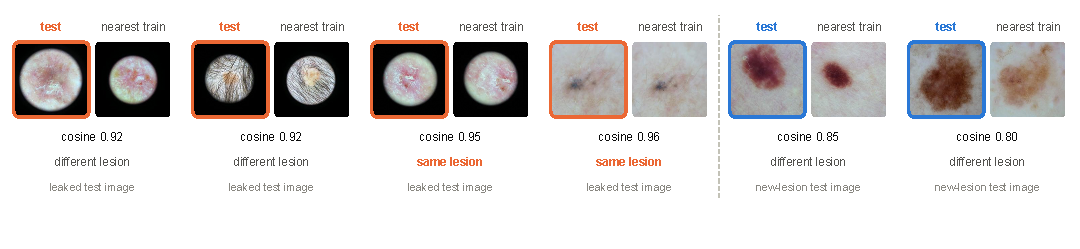
\includegraphics[width=\textwidth]{FigS1_proximity_examples}}{\fbox{FigS1\_proximity\_examples.pdf}}
\caption{Exploratory nearest-neighbor examples (randomly drawn leaked test images, seed 20261106, not selected): each
test image with its nearest training image in the frozen embedding space.}
\end{figure}
\end{document}
